\documentclass[./\jobname.tex]{subfiles}
\begin{document}
\chapter {Experiment 2: Adaptive Number of Kernels}
\label{chap:experimet_2}

Although the parallel algorithm is effectively faster, the quality of the achieved solution is still not good enough. A common inaccuracy, especially with the testbed \gls{pde} 0A is that not all Gauss ``bumps'' are represented in the approximation, as described in chapter \ref{chap: experiment_0_pde_0A}. A possible method to compensate that could be to adapt the number of kernels along the solving process, instead of arbitrarily using 5 kernels. 

\section{Hypotheses}

The idea tested in this chapter is an adaptive scheme for the number of kernels used, which is directly linked to the search dimensionality of the optimisation problem. 

This new concept requires a convergence based halting criterion in the JADE algorithm, which is not included in the algorithm before. The pseudocode \ref{algo: pajade} in the \mbox{appendix \ref{chap:pseudocode_pajade}} is extended by a so called ``state detector''. Ideally, the state detector (code-lines 37 to 40) should stop the overall optimisation loop as soon as the algorithm has converged and before the function evaluation budget is exceeded. Generally, this is done by checking if the function value has not changed for a certain amount of generations. The state detector introduces a new parameter. The \gls{dt} represents the number of generations over which the best function value must remain unchanged. It can also be thought of as a buffer-time that allows the \gls{de} parameters F and CR to self-adapt. Further, the minError parameter has a new purpose. This is the minimal difference that the function value is allowed to change over \gls{dt} generations, without resetting the counter for \gls{dt}. 

The new paJADE is wrapped into the memetic framework, already used in the chapters before. A flowchart of the process in shown in figure \ref{fig:uml_flow_adaptive_scheme}. The corresponding pseudocode \ref{algo: memeticpJADEadaptive} in the appendix describes the implementation.

The algorithm always starts with one kernel. From there on, the number of kernels is increased. After the ``state detector'' has stopped the paJADE, the \gls{ds} is employed on the best individual of the last population. If the last JADE/DS cycle was able to improve the function value, it is assumed that the best solution for that dimensionality is found. Thus, to further improve the approximation quality, the number of kernels must be increased. If the function value could not be decreased, a restart around the previous best population is performed. Since the number of kernels is always increased by one, the previous best population must have one kernel less. 

\begin{figure}[H]
	\centering
	\noindent\adjustbox{max width=0.9\linewidth}{
		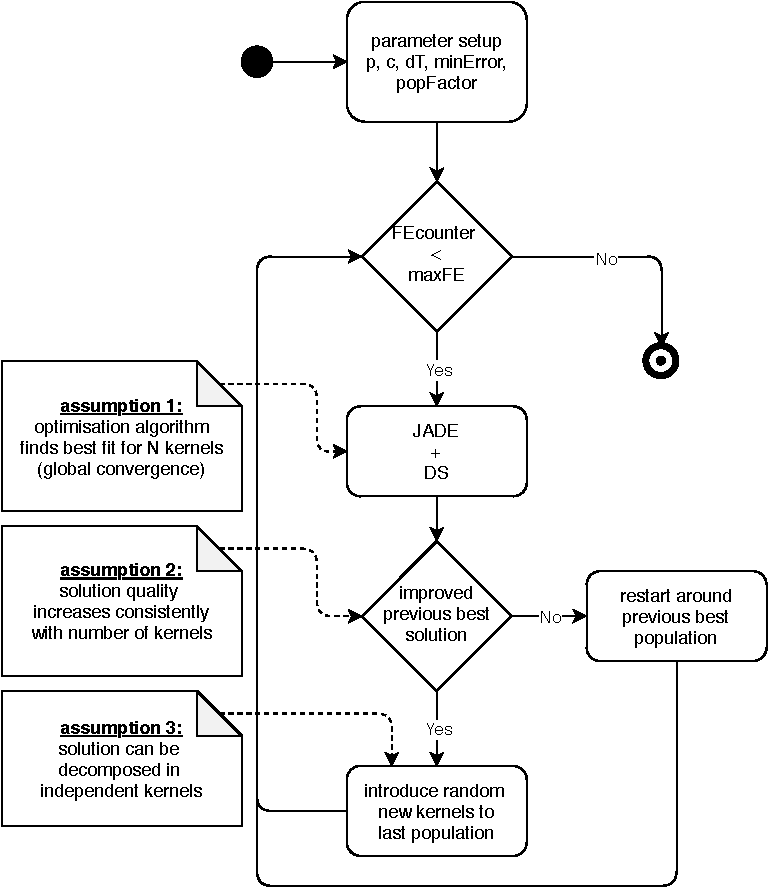
\includegraphics[width=\textwidth]{../../code/uml_diag/adaptive_kernels_flowchart.pdf}
	}
	\unterschrift{Flowchart of the adaptive kernel scheme.}{}{}
	\label{fig:uml_flow_adaptive_scheme}
\end{figure}

This adaptive scheme operates under 3 strong assumptions. To reduce their possible negative impact, corresponding counter-strategies are implemented. 
\begin{itemize}
	\item \underline{\textbf{Assumption 1:}} The optimisation algorithm (JADE + \gls{ds}) finds (a close approximation to) the global optimum. This would be the best approximation of the solution by $N$ kernels. Obviously, this property is not necessarily true. Currently, only a very limited amount of research papers exist, that discuss global convergence properties of \gls{de} (\cite{hu_sufficient_2013}, \cite{opara_differential_2019}). To counteract this assumption, restarts are performed. 
	\item \underline{\textbf{Assumption 2:}} The theoretically best achievable solution quality increases with the number of kernels. After a maximum number of kernels is reached, the quality can not be surpassed. Based on this assumption, the algorithm starts with one kernel and the dimensionality increases by only one kernel at a time. To catch the point after which too many kernels are used, the dimensionality reduction step is introduced. Generally, the maximum number of kernels is not known except for \gls{pde} 0A and \gls{pde} 6. 
	\item \underline{\textbf{Assumption 3:}} The best approximation of e.g. 3 kernels to a particular problem is independent of the best approximation by 4 kernels. This means that from 3 to 4 kernels simply a new kernel is introduced while not altering the other 3. Again, this is not true for every \gls{pde}. Preliminary experiments on \gls{pde} 0A have confirmed this assumption, while on other \gls{pde}s, like \gls{pde} 2, the solution can not simply be decomposed into independent kernels. 
	
	The concept is similar to the one explained in \cite{chaquet_solving_2012}. They start the approximation process by optimising the first harmonic. During the search for the second harmonic, the first one is fixed in place. 
	
	In this algorithm, the first kernels are allowed to change. When introducing a new random kernel, it is simply appended to the ever evolving $\mathbf{p_{apx}}$ vector. Thus, the search for the 4th kernel starts where the best approximation for 3 kernels was found, but since the earlier kernels are allowed to readapt, other solutions can be retrieved.
\end{itemize} 

This chapter discusses the question if this strategy is an effective method to increase the quality of obtained solutions. Also, the time and memory aspects are investigated. 

\section{Experiment Setup}

Again, as in the experiments before, machine 1 runs at $10^4$ \gls{nfe} and machine 2 performs $10^6$ \gls{nfe}. The time- and memory-comparison are done on machine 1. The number of kernels is adapted, but the algorithm starts with 1 \gls{gak}. Thus, the dimension is 4 and the population size is 8. The population size gets corrected if the number of kernels changes. The Wilcoxon test from appendix \ref{chap:apendix_post_proc} investigates the statistical significance. 

The two new parameters \gls{dt} and minError must be set. The minError is again set to 0. The delay time \gls{dt} is set to 100. When the function value could not be improved over the course of 100 consecutive generations, a new kernel is introduced. This choice is rather arbitrary and depending on the \gls{pde}, different values might be more successful. However, this property is not analysed in the current experiment.

\section{Result}
\label{chap:results_ex2}

Similar to the experiments before, the two images \ref{fig:pajade_time_boxplot} and \ref{fig:pajade_memory_boxplot} illustrate the time and memory usage of the described kernel adaptive JADE. The data to both plots is obtained on machine 1 at $10^4$ \gls{nfe}. \gls{pde} 7 takes the longest to solve, about 8.5 times longer than the \gls{fem} solver. Contrary, \gls{pde} 3 is solved the fastest, where the \gls{ci} solver only needs about a quarter of the time used by \gls{fem} solver. The memory effort of the \gls{ci} solver over all testbed problems is between 0.5 and 2.5 percent of the memory needed by the \gls{fem} solver. 

\begin{figure}[H]
	\centering
	\noindent\adjustbox{max width=0.66\linewidth}{
		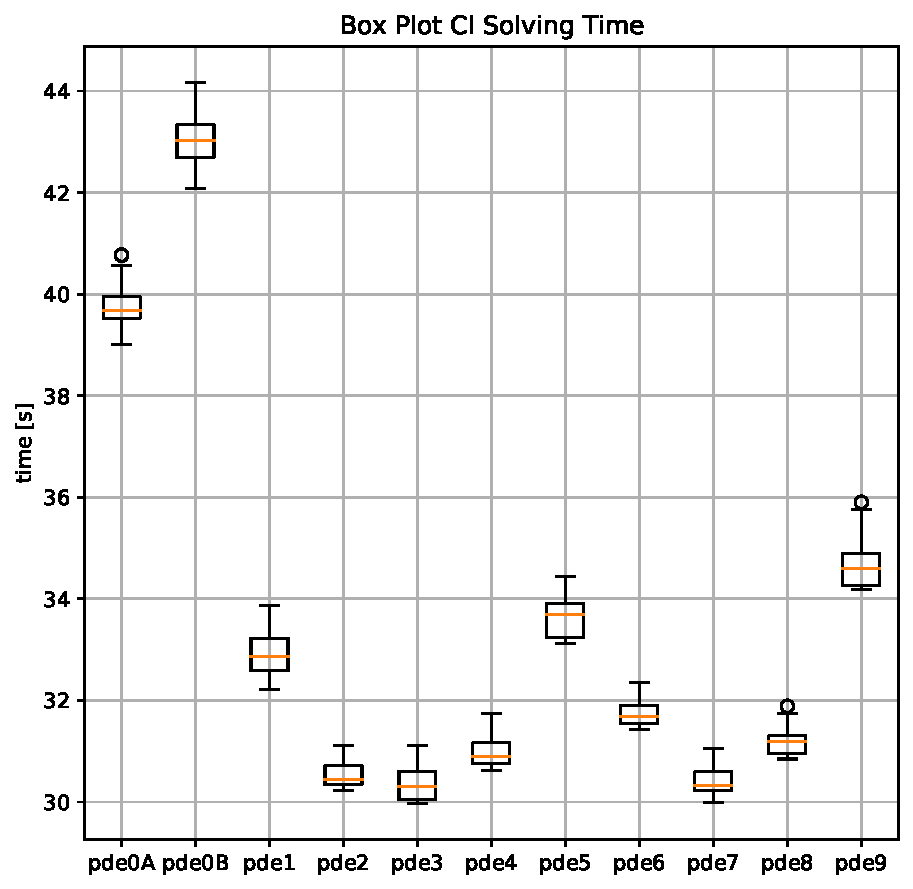
\includegraphics[width=\textwidth]{../../code/experiments/experiment_2/time_boxplot_ci_exp2.pdf}
	}
	\unterschrift{Relative solving time results of parallel memetic JADE with adaptive kernels after $10^4$ \gls{nfe}.}{}{}
	\label{fig:pajade_time_boxplot}
\end{figure}


\begin{figure}[H]
	\centering
	\noindent\adjustbox{max width=0.66\linewidth}{
		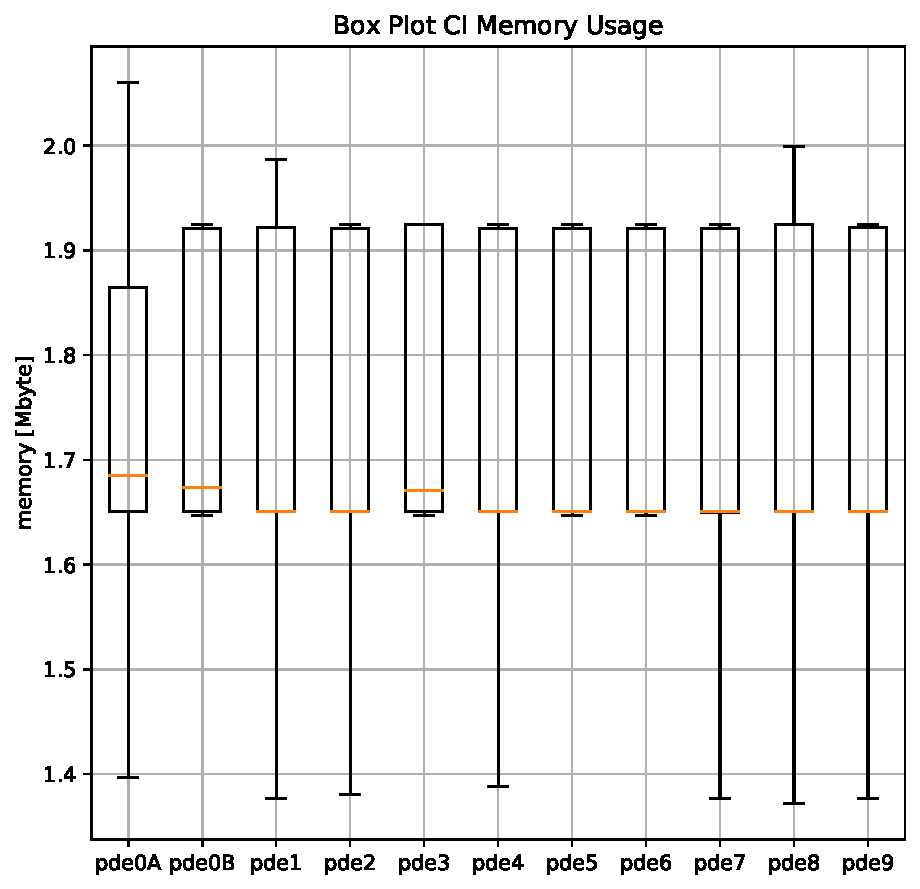
\includegraphics[width=\textwidth]{../../code/experiments/experiment_2/mem_boxplot_ci_exp2.pdf}
	}
	\unterschrift{Relative memory usage results of parallel memetic JADE with adaptive kernels after $10^4$ \gls{nfe}.}{}{}
	\label{fig:pajade_memory_boxplot}
\end{figure}

The table \ref{tab:compare_mpj_mpja_10^6} shows the L2 norm data obtained by the adaptive JADE and compares them against the results from the parallel JADE. The Wilcoxon test indicates mixed results. The adaptive kernel scheme works fine on the \gls{pde} 0A, but it also produces significantly worse results on the problems \gls{pde} 2, 3, 4 and 7. 

\begin{table}[H]
	\centering
	\noindent\adjustbox{max width=\linewidth}{
		\begin{tabular}{|c|c|c|c|c|l|}
			
			\hline
			\rowcolor[HTML]{\farbeTabA}
			
			Algorithm & \multicolumn{2}{|c|}{parallel JADE $10^6$ \gls{nfe}} & \multicolumn{2}{|c|}{adaptive JADE $10^6$ \gls{nfe}} & \\ \hline
			stat & mean & median & mean & median & Wilcoxon Test \\ \hline \hline
			\gls{pde} 0A & 0.6939 $\pm$ 0.6635 & 0.9243 & 9.694E-16 $\pm$ 1.486E-16 & 9.255E-16 & sig. better \\ \hline
			\gls{pde} 0B & 0.2809 $\pm$ 0.3071 & 0.2035 & 0.2380 $\pm$ 0.0572 & 0.2607 & unsig. undecided \\ \hline
			\gls{pde} 1 & 0.0239 $\pm$ 0.0467 & 0.0146 & 0.0116 $\pm$ 0.0061 & 0.0084 & unsig. better \\ \hline
			\gls{pde} 2 & 0.0300 $\pm$ 0.0157 & 0.0255 & 0.0735 $\pm$ 0.0358 & 0.1034 & sig. worse \\ \hline
			\gls{pde} 3 & 0.0371 $\pm$ 0.0206 & 0.0295 & 0.1731 $\pm$ 0.0395 & 0.1822 & sig. worse \\ \hline
			\gls{pde} 4 & 0.0505 $\pm$ 0.0121 & 0.0481 & 0.0707 $\pm$ 0.0053 & 0.0720 & sig. worse\\ \hline
			\gls{pde} 5 & 1.2030 $\pm$ 0.0465 & 1.2053 & 122.6312 $\pm$ 372.5676 & 1.1643 & unsig. undecided \\ \hline
			\gls{pde} 6 & 0.5814 $\pm$ 1.3550 & 1.266E-17 & 0.4428 $\pm$ 1.0980 & 1.266E-17 & unsig. undecided \\ \hline
			\gls{pde} 7 & 0.0228 $\pm$ 0.0025 & 0.0226 & 0.0513 $\pm$ 0.0442 & 0.0231 & sig. worse \\ \hline
			\gls{pde} 8 & 0.2167 $\pm$ 0.0017 & 0.2169 & 0.2144 $\pm$ 0.0044 & 0.2128 & unsig. better \\ \hline
			\gls{pde} 9 & 0.0426 $\pm$ 0.0115 & 0.0463 & 0.0483 $\pm$ 0.0149 & 0.0468 & unsig. worse \\ \hline
			
		\end{tabular}
	}
	\unterschrift{Comparison of the achieved L2 norm by the pJADE and the paJADE at $10^6$ \gls{nfe}. The pJADE data is directly taken from table \ref{tab:compare_parallel_serial_jade_10^6}.}{}{}
	\label{tab:compare_mpj_mpja_10^6}
\end{table}

Since the number of kernels is not predefined, the resulting solution may have any amount of kernels. This is also a random variable, and the results are shown in the boxplot \ref{fig:pajade_kernels_boxplot} below. As expected, this varies between different testbed problems, but it can not be less than 1 kernel. 

\begin{figure}[H]
	\centering
	\noindent\adjustbox{max width=0.66\linewidth}{
		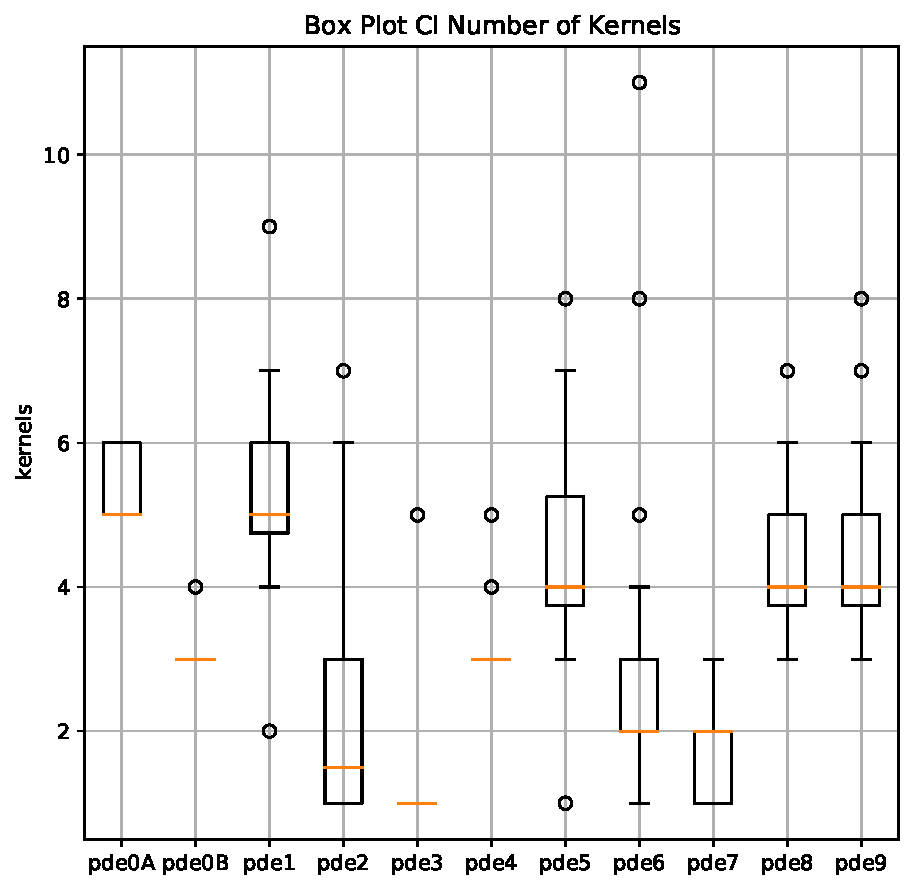
\includegraphics[width=\textwidth]{../../code/experiments/experiment_2/kernels_boxplot_ci_exp2.pdf}
	}
	\unterschrift{Number of kernels of the proposed solution by the paJADE per \gls{pde} at $10^6$ \gls{nfe}}{}{}
	\label{fig:pajade_kernels_boxplot}
\end{figure}


\section{Discussion}

This chapter analyses the presented results from section \ref{chap:results_ex2}. The time and memory usage is discussed. The significantly better results on \gls{pde} 0A are investigated. The adaptive kernel scheme performs significantly worse on the testbed problems \gls{pde} 2, 3, 4, and 7. Therefore the $minError$ parameter is adapted and the results are critically examined. 

\subsection{Solving Time}

This new adaptive strategy can significantly decrease the time that is necessary to solve any \gls{pde} of the testbed. This follows from the solving time box plot in figure \ref{fig:pajade_time_boxplot}. This effect can be explained by the reduction of the dimension and the adaptive population size. Depending on the number of kernels, the population can grow. It always starts with 1 kernel and therefore the size of the population is 8. The boxplot shows that this breaks the pattern of simpler and more complex \gls{pde}s that is exhibited in the previous experiments.

\subsection{Memory Usage}
The adaptive approach also leads to a reduction in the memory usage, as described by the memory boxplot in figure \ref{fig:pajade_memory_boxplot}. The same explanation that describes the solving time reduction can be applied here: smaller populations need less memory to be stored. Since not all \gls{pde}s result in the same dimension, the memory consumption over all testbed problems is not the same. Further, the adaptive scheme dismantles the linear scaling of memory usage with increasing \gls{nfe}. 

\subsection{PDE 0A}
\label{chap:ex2_discussion_pde0a}
As noted before, the testbed \gls{pde} is especially designed to be solved by 5 \gls{gak}. The common problem, that not all kernels are established, is solved by the adaptive strategy. The kernel boxplot in figure \ref{fig:pajade_kernels_boxplot} shows that all 20 replications generate at least 5 kernels. However, some solutions are composed of 6 kernels, but this has only a limited effect on the numerical value of the solution quality. Generally, 6 kernels tend to produce worse solutions. The results by the \gls{ci} solver can even compete with the \gls{fem} solver results from table \ref{tab:fem_sol_quality}.

There are mainly three things that can happen to the unnecessary kernel: 
\begin{itemize}
	\item Put the kernel far outside of $\Omega$ with $c_0$ and $c_1$, so that the influence within the domain is negligible.
	\item Reduce the scaling factor $\varphi$ to near 0, therefore the kernel has a small influence compared to the others.
	\item Increase the exponent $\gamma$ so that the kernel is very sharp and the influence dies out rapidly with $r$.
\end{itemize}

Figure \ref{fig:paJADE_pde0a_6kernel} shows the 3D plot of two separate unnecessary kernels produced by the adaptive memetic pJADE. A kernel with increased $\gamma$ is not included in the dataset.

\begin{figure}[H]
	\centering
	\begin{subfigure}[b]{0.42\linewidth}
		\centering
		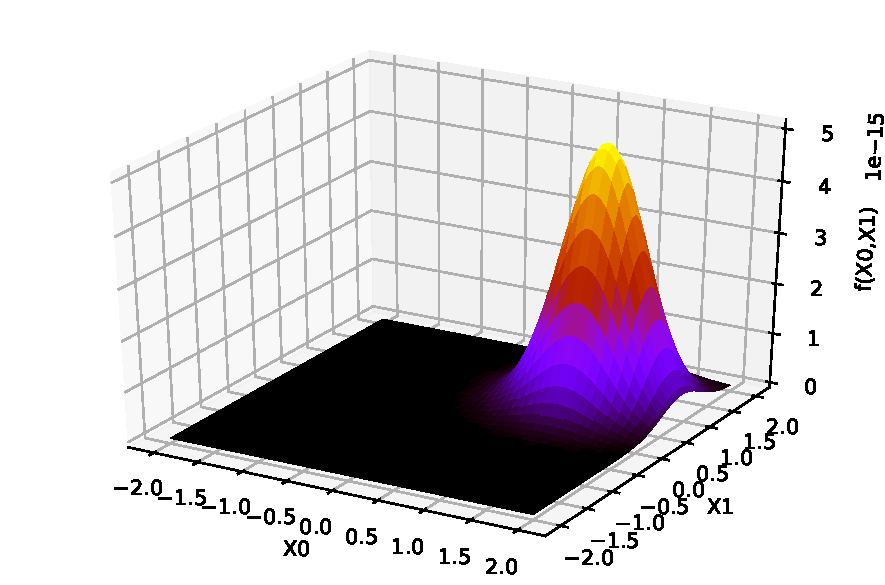
\includegraphics[width=1\textwidth]{../../code/experiments/experiment_2/cipde0a_kernel6_small.pdf}
		\caption{small scaling factor \\ $\varphi=5.066\cdot 10^{-15}$ \\ $f(c_0,c_1)=5\cdot10^{-15}$}
		\label{fig:paJADE_pde0a_6kernel_out}
	\end{subfigure}% 
	%
	\begin{subfigure}[b]{0.42\linewidth}
		\centering
		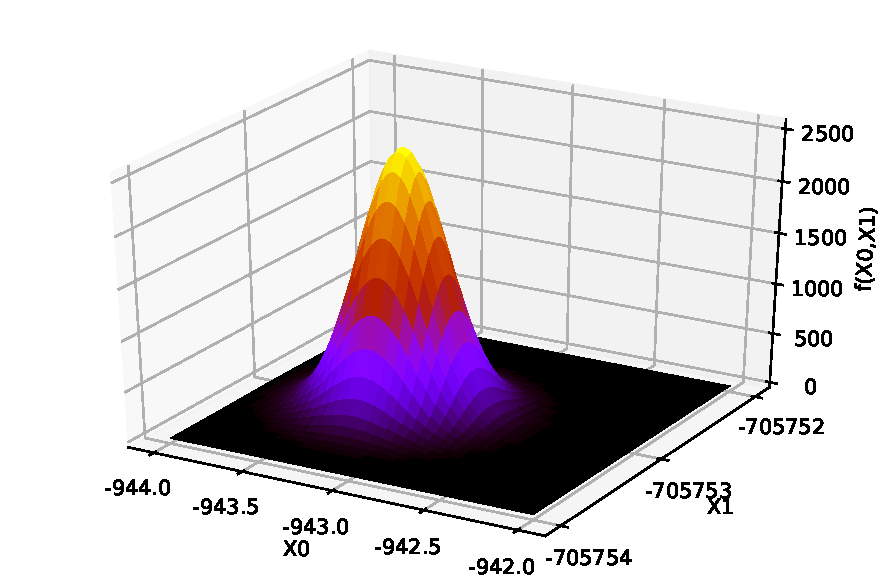
\includegraphics[width=1\textwidth]{../../code/experiments/experiment_2/cipde0a_kernel6_out.pdf}
		\caption{outside the domain $\Omega$\\ $c_0=-943.237$ \\ $c_1=-705753.067$.}
		\label{fig:paJADE_pde0a_6kernel_small}
	\end{subfigure}%
	\unterschrift{3D plot and comparison of unnecessary 6\textsuperscript{th} kernels on \gls{pde} 0A.}{}{}%
	\label{fig:paJADE_pde0a_6kernel}
\end{figure}


\subsection{Significantly Worse Quality}
\label{chap:pde 2 3 4 7}
The Wilcoxon significance test of table \ref{tab:compare_mpj_mpja_10^6} shows that the adaptive scheme is worse for the \gls{pde}s 2, 3, 4 and 7. The boxplot \ref{fig:pajade_kernels_boxplot} shows that on these test problems the solver frequently results in a smaller number of kernels, where the majority of runs even produce less than 5 \gls{gak}. This phenomenon points towards a shared problem where the solver does not increase the number of kernels consistently. 

Figure \ref{fig:pajade_pde2347_kernels_l2norm} plots the solution quality against its number of kernels. It is clearly shown that on these \gls{pde}s, more kernels strongly correlate with a better quality. 

\begin{figure}[H]
	\centering
	\noindent\adjustbox{max width=0.7\linewidth}{
		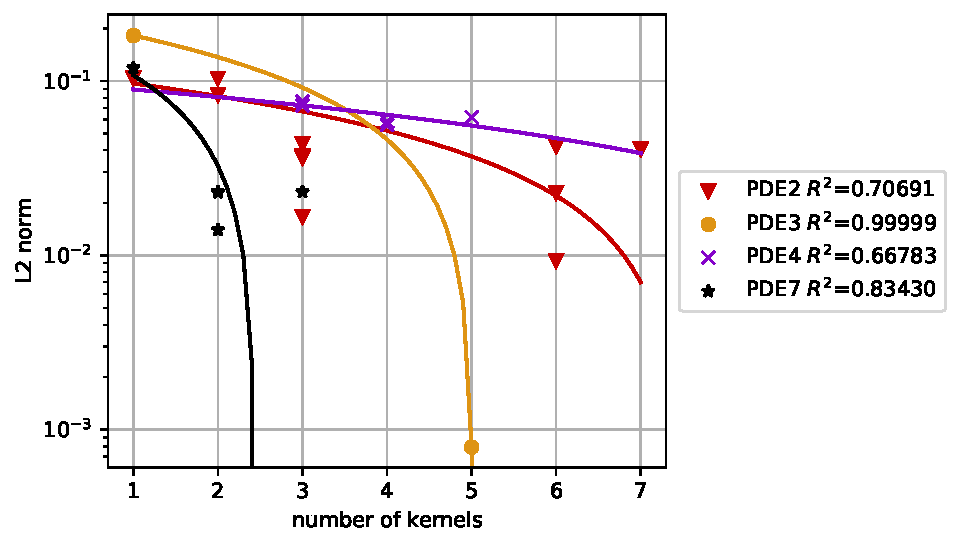
\includegraphics[width=\textwidth]{../../code/experiments/experiment_2/pde_2_3_4_7_kernels_vs_l2norm.pdf}
	}
	\unterschrift{Semi-logarithmic plot of the correlation between the L2 norm and the number of kernels. The results are taken at $10^6$ \gls{nfe} on the \gls{pde}s 2, 3, 4 and 7. The corresponding $R^2$ values of the linear regression are denoted.}{}{}
	\label{fig:pajade_pde2347_kernels_l2norm}
\end{figure}

It seems that JADE exploits some areas long enough so that it does not terminate due to convergence. Thus, the number of kernels is not increased, which leads to a poor approximation quality. The kernel bar plot of the best and the worst replication for these 4 \gls{pde}s is shown in the appendix \ref{chap: appendix kernel bar plot} and confirms this hypothesis. A simple solution to mitigate this issue might be to adjust the parameters of the ``state-detector''. In this experiment, $minError = 0$ is used, however it might be beneficial to allow small changes in the function value and still terminate. 

\textbf{\underline{Parameter Adaption: $minError$}} 

In this ``sub-experiment'' the effect of increasing the $minError$ parameter is examined. Therefore, the same algorithm is rerun on the \gls{pde}s 2, 3, 4 and 7 at four different $minError$ levels. Again, 20 replications are done. It is expected that the average number of kernels is increased. Simultaneously, the approximation quality should become better. 

As expected, the average number of kernels in the solution gets increased. This is confirmed by the plot in figure \ref{fig:subexperiment_pde2347_minerror_kernelNR}. Figure \ref{fig:subexperiment_pde2347_minerror_l2norm} shows the connection between the median L2 norm and the $minError$. The distance to the analytical solution decreases on \gls{pde} 2 and 3. However, this does not improve the results of \gls{pde} 4 and 7, where the quality stays roughly on the same level. This is supported statistically by the Wilcoxon test in table \ref{tab:statistical_test_minError}.

\begin{figure}[H]
	\centering
	\begin{subfigure}[b]{0.5\linewidth}
		\centering
		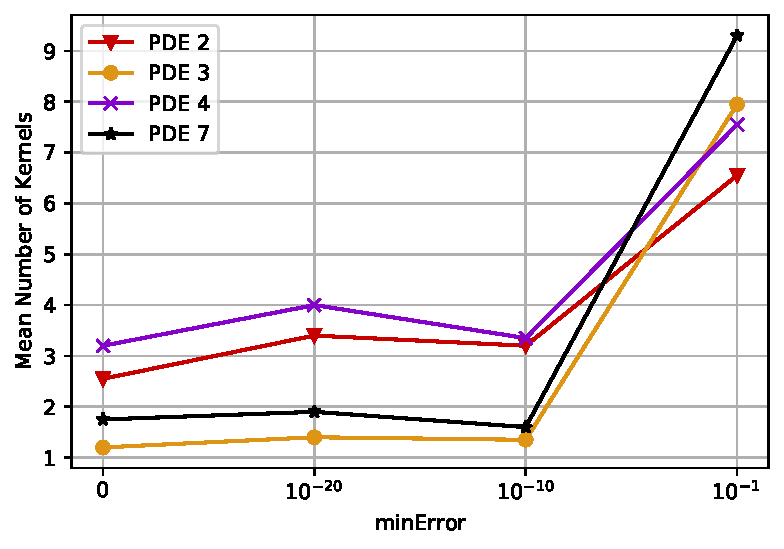
\includegraphics[width=1\textwidth]{../../code/experiments/misc/pde2347_minError_kernelNR.pdf}
		\caption{Plot of the mean number of kernels against the $minError$.}
		\label{fig:subexperiment_pde2347_minerror_kernelNR}
	\end{subfigure}% 
	%
	\begin{subfigure}[b]{0.52\linewidth}
		\centering
		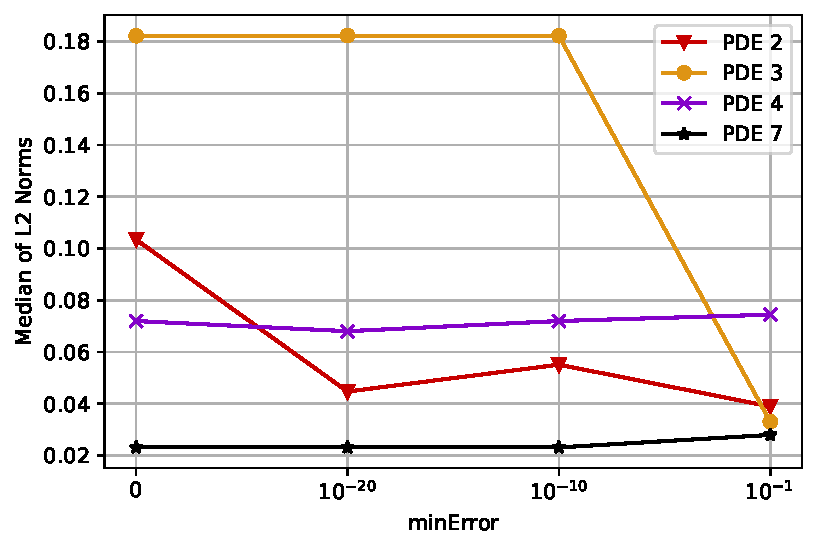
\includegraphics[width=1\textwidth]{../../code/experiments/misc/pde2347_minError_L2norm.pdf}
		\caption{Plot of the median L2 norm against the $minError$.}
		\label{fig:subexperiment_pde2347_minerror_l2norm}
	\end{subfigure}%
	\unterschrift{Comparison of $minError$ against the number of kernels and the achieved solution quality. }{}{}%
	\label{fig:subexperiment_pde2347_minerror}
\end{figure}

\begin{table}[H]
	\centering
	\noindent\adjustbox{max width=\linewidth}{
		\begin{tabular}{|c|c|c|c|c|l|}
			
			\hline
			\rowcolor[HTML]{\farbeTabA}
			
			Setup & \multicolumn{2}{|c|}{$minError = 0$; $10^6$ \gls{nfe}} & \multicolumn{2}{|c|}{$minError = 10^{-1}$; $10^6$ \gls{nfe}} & \\ \hline
			stat & mean & median & mean & median & Wilcoxon Test \\ \hline \hline
			\gls{pde} 2 & 0.0735 $\pm$ 0.0358 & 0.1034 & 0.0418 $\pm$ 0.0156 & 0.0389 & sig. better \\ \hline
			\gls{pde} 3 & 0.1731 $\pm$ 0.0395 & 0.1822 & 0.0455 $\pm$ 0.0406 & 0.0331 & sig. better \\ \hline
			\gls{pde} 4 & 0.0707 $\pm$ 0.0053 & 0.0720 & 0.0726 $\pm$ 0.0080 & 0.0744 & unsig. worse \\ \hline
			\gls{pde} 7 & 0.0513 $\pm$ 0.0442 & 0.0231 & 0.0287 $\pm$ 0.0045 & 0.0279 & unsig. undecided \\ \hline
			
		\end{tabular}
	}
	\unterschrift{Statistical comparison of the achieved L2 norm by paJADE with $minError = 0$ and $minError = 10^{-1}$ after $10^6$ \gls{nfe}. The data with $minError = 0$ is directly taken from table \ref{tab:compare_mpj_mpja_10^6}.}{}{}
	\label{tab:statistical_test_minError}
\end{table}


Although the results on \gls{pde} 2 and 3 do get significantly better, the adaptive process with greater $minError$ introduces a larger spread of the results - both in the number of kernels and in the reached L2 norm. This can be seen in figure \ref{fig:subexperiment_pde2347_kernels_l2norm}. Compared to the same plot at $minError = 0$ (figure \ref{fig:pajade_pde2347_kernels_l2norm}), the coefficient of determination $R^2$ is smaller, indicating a poor correlation. 

\begin{figure}[H]
	\centering
	\noindent\adjustbox{max width=0.7\linewidth}{
		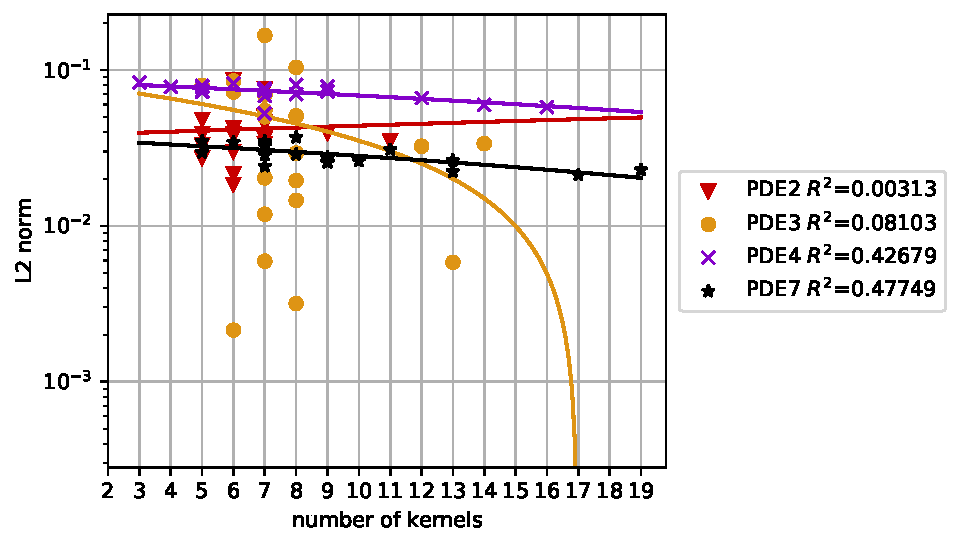
\includegraphics[width=\textwidth]{../../code/experiments/misc/pde2347_L2norm_kernelNR.pdf}
	}
	\unterschrift{Semi-logarithmic plot of the correlation between the L2 norm and the number of kernels. The results are produced with a $minError = 10^-1$ after $10^6$ \gls{nfe}.}{}{}
	\label{fig:subexperiment_pde2347_kernels_l2norm}
\end{figure}

Because JADE is terminated earlier, the exploitation is not as progressed. This trade-off needs to be managed by setting the ``state-detector''-parameters. A small $minError$ ensures that the exploitation is progressed sufficiently, but it exceeds the \gls{nfe} budget before the number of kernels is increased. Contrary, larger $minError$-values terminate faster and increase the number of kernels, but the solution is not fully exploited. 

\subsection{PDE 5}

The results presented in table \ref{tab:compare_mpj_mpja_10^6} shows an interesting observation for the testbed problem 5. The mean L2 norm of the adaptive scheme is very large, but the median is slightly smaller than the median of the non-adaptive JADE. The Wilcoxon test reveals an insignificant difference, which hints that the adaptive scheme includes some very large outliers. This is demonstrated by comparing the box plots of both L2 norm distributions in figure \ref{fig:paJADE_pde5_l2norm_boxplot}. The same data is shown twice, with and without the outlier. 

\begin{figure}[H]
	\centering
	\begin{subfigure}[b]{0.4\linewidth}
		\centering
		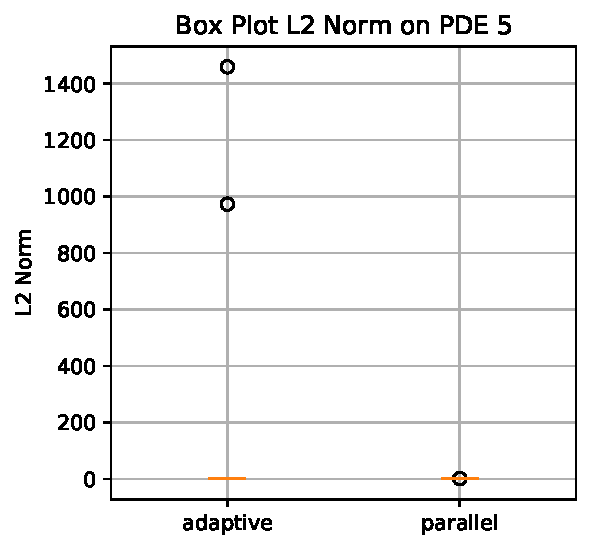
\includegraphics[width=1\textwidth]{../../code/experiments/experiment_2/pde5_L2_norm_boxplot.pdf}
		\caption{Boxplot of \gls{pde} 5 solution quality with outlier. }
		\label{fig:paJADE_pde5_l2norm_boxplot}
	\end{subfigure}% 
	%
	\begin{subfigure}[b]{0.39\linewidth}
		\centering
		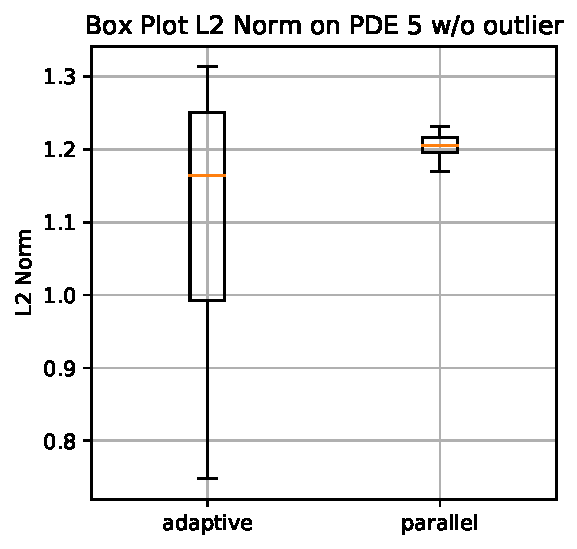
\includegraphics[width=1\textwidth]{../../code/experiments/experiment_2/pde5_L2_norm_boxplot_wo_outlier.pdf}
		\caption{Boxplot of \gls{pde} 5 solution quality without outlier. }
		\label{fig:paJADE_pde5_l2norm_boxplot_cleared}
	\end{subfigure}%
	%
	\unterschrift{Boxplot of solution quality on \gls{pde} 5 with a budget of $10^6$ \gls{nfe}. Comparison of distribution with and without outliers. }{}{}%
	\label{fig:paJADE_pde5_l2norm_boxplot_comparison}
\end{figure}

The approximate solution of the outlier is shown in the two 3D plots in figure \ref{fig:paJADE_pde5_3D_plot_outlier} below. Evidently, both results have nothing in common with the actual solution from figure \ref{fig:pde5_analytical_solution_2}. In general, it can be said that the adaptive scheme exhibits a greater spread in the quality of the solution. 

\begin{figure}[H]
	\centering
	\begin{subfigure}[b]{0.3333\linewidth}
		\centering
		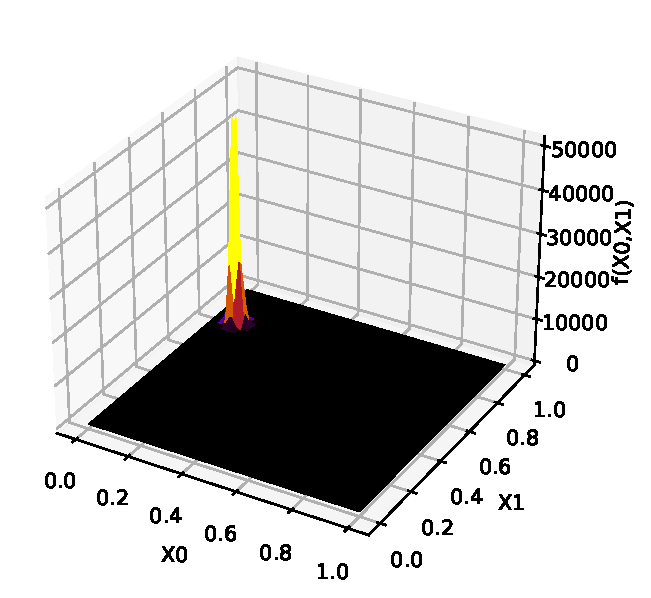
\includegraphics[width=1\textwidth]{../../code/experiments/experiment_2/pde5_outlier1_3D_plot.pdf}
		\caption{3D plot of first \\outlier on \gls{pde} 5}
		\label{fig:paJADE_pde5_outlier0}
	\end{subfigure}% 
	%
	\begin{subfigure}[b]{0.3333\linewidth}
		\centering
		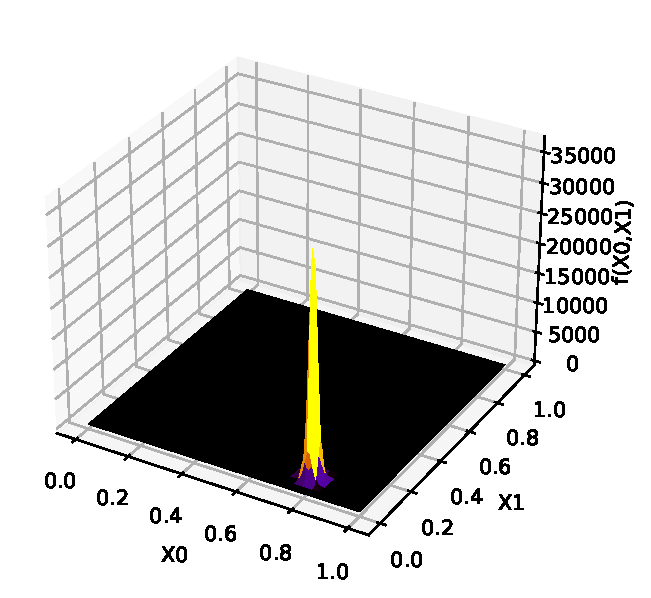
\includegraphics[width=1\textwidth]{../../code/experiments/experiment_2/pde5_outlier2_3D_plot.pdf}
		\caption{3D plot of second \\outlier on \gls{pde} 5}
		\label{fig:paJADE_pde5_outlier1}
	\end{subfigure}%
	%
	\begin{subfigure}[b]{0.3333\linewidth}
		\centering
		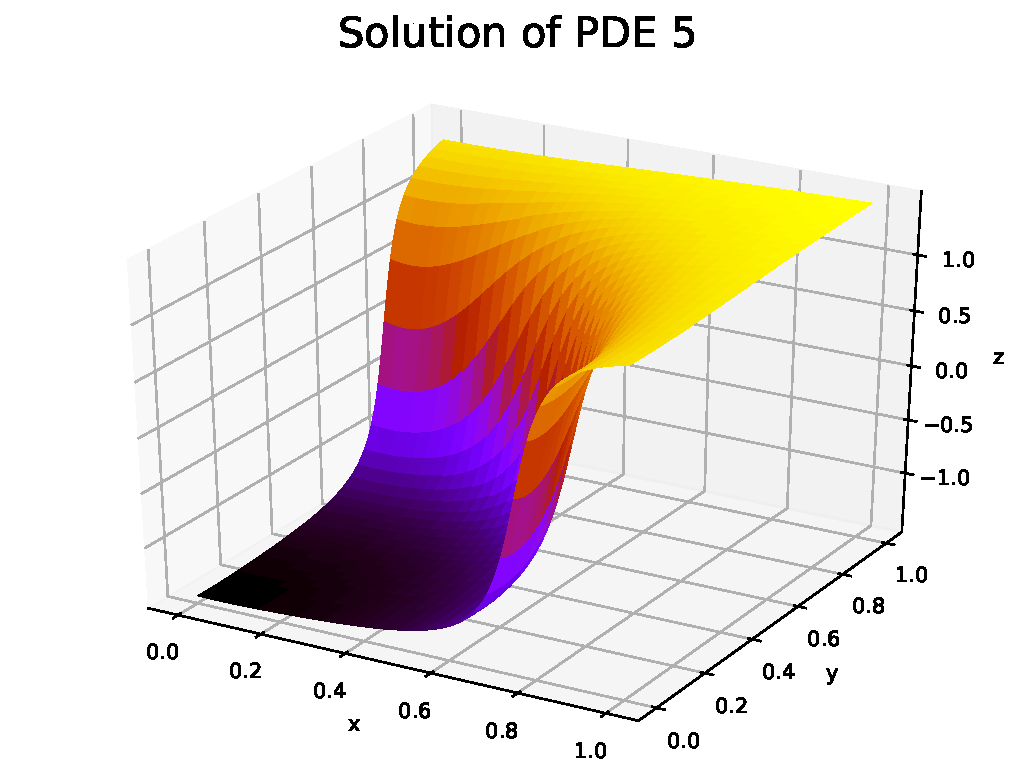
\includegraphics[width=1\textwidth]{../../code/testbed/pde5/sol_pde_5.pdf}
		\caption{analytical solution \\to \gls{pde} 5.}
		\label{fig:pde5_analytical_solution_2}
	\end{subfigure}%
	\unterschrift{3D plot of the outlier solution produced by the adaptive kernel scheme on \gls{pde} 5 after $10^6$ \gls{nfe}.}{}{}%
	\label{fig:paJADE_pde5_3D_plot_outlier}
\end{figure}

Both outliers have a very similar structure. This might indicate that JADE diverges to areas where the fitness function does not give a proper signal towards the optimum. The adaptive strategy can not improve the results on \gls{pde} 5. A second possibility would be to use a different kernel type. 


\subsection{PDE 6}

The testbed \gls{pde} 6 could theoretically be solved exactly by a single \gls{gak}. As the Wilcoxon test shows, the adaptive kernel method does not improve the results significantly. This is confirmed in the subsequent boxplot of figure \ref{fig:paJADE_pde6_l2norm_boxplot_comparison}. Even good solutions are made of more than one kernel, as the boxplot in \ref{fig:pajade_kernels_boxplot} indicates. This means that the adaptive kernel strategy is not successful on \gls{pde} 6. JADE terminates to early and introduces more kernels. The influence of these unnecessary kernels must be minimised by the same strategies as with \gls{pde} 0A as presented in chapter \ref{chap:ex2_discussion_pde0a}.

\begin{figure}[H]
	\centering
	\begin{subfigure}[b]{0.381\linewidth}
		\centering
		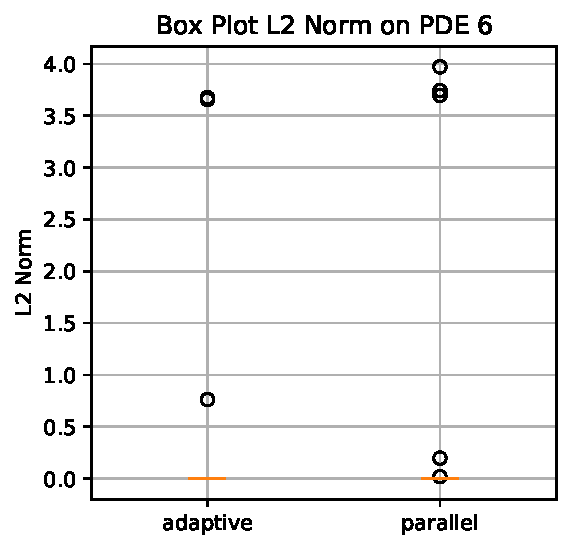
\includegraphics[width=1\textwidth]{../../code/experiments/experiment_2/pde6_L2_norm_boxplot.pdf}
		\caption{Boxplot of \gls{pde} 6 L2 norm results with fliers.}
		\label{fig:paJADE_pde6_l2norm_boxplot}
	\end{subfigure}% 
	%
	\begin{subfigure}[b]{0.4\linewidth}
		\centering
		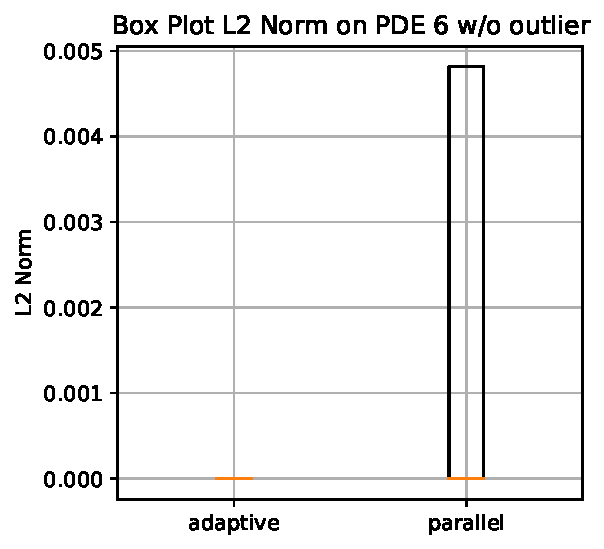
\includegraphics[width=1\textwidth]{../../code/experiments/experiment_2/pde6_L2_norm_boxplot_wo_outlier.pdf}
		\caption{Boxplot of \gls{pde} 6 L2 norm results without fliers.}
		\label{fig:paJADE_pde6_l2norm_boxplot_cleared}
	\end{subfigure}%
	\unterschrift{Comparison of the L2 norm reached by the paJADE and a non-adaptive pJADE on \gls{pde} 6 after $10^6$ \gls{nfe}.}{}{}%
	\label{fig:paJADE_pde6_l2norm_boxplot_comparison}
\end{figure}

Besides the good results, there are two recurring bad solutions as seen in figure \ref{fig:paJADE_pde6_3D_plot_outlier}. Their 3D plot shows no resemblance with the actual solution from figure \ref{fig:pde6_analytical_solution}. The fact that these obviously bad approximations happen multiple times indicates that JADE converges to these local optima. 

\begin{figure}[H]
	\centering
	\begin{subfigure}[b]{0.333\linewidth}
		\centering
		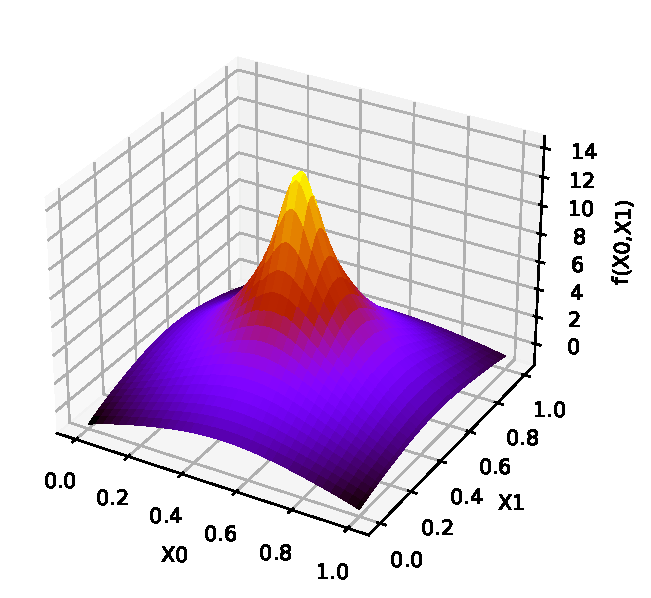
\includegraphics[width=1\textwidth]{../../code/experiments/experiment_2/pde6_3D_plot_outlier1.pdf}
		\caption{outlier 8 \gls{gak}\\ kernel bar plot figure \ref{fig:paJADE_pde6_kernel_bar_plot_outlier1}}
		\label{fig:pajade_pde6_3D_plot_outlier1}
	\end{subfigure}% 
	%
	\begin{subfigure}[b]{0.333\linewidth}
		\centering
		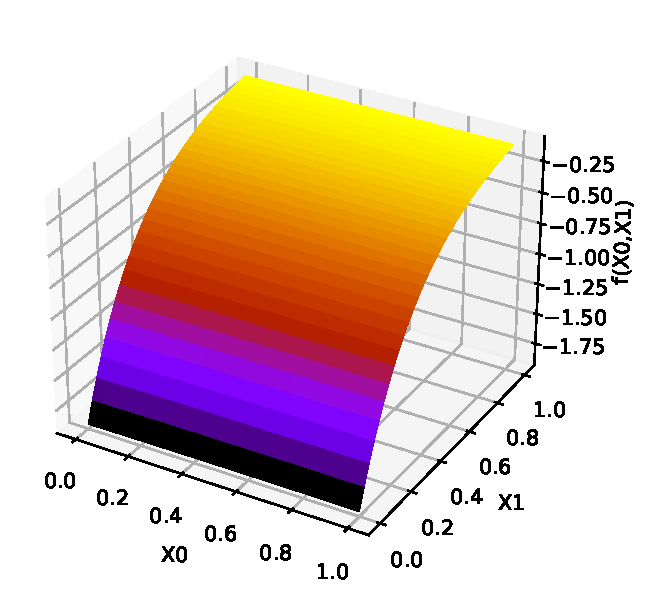
\includegraphics[width=1\textwidth]{../../code/experiments/experiment_2/pde6_3D_plot_outlier2.pdf}
		\caption{outlier 1 \gls{gak}\\ kernel bar plot figure \ref{fig:paJADE_pde6_kernel_bar_plot_outlier2}}
		\label{fig:pajade_pde6_3D_plot_outlier2}
	\end{subfigure}%
	%
	\begin{subfigure}[b]{0.333\linewidth}
		\centering
		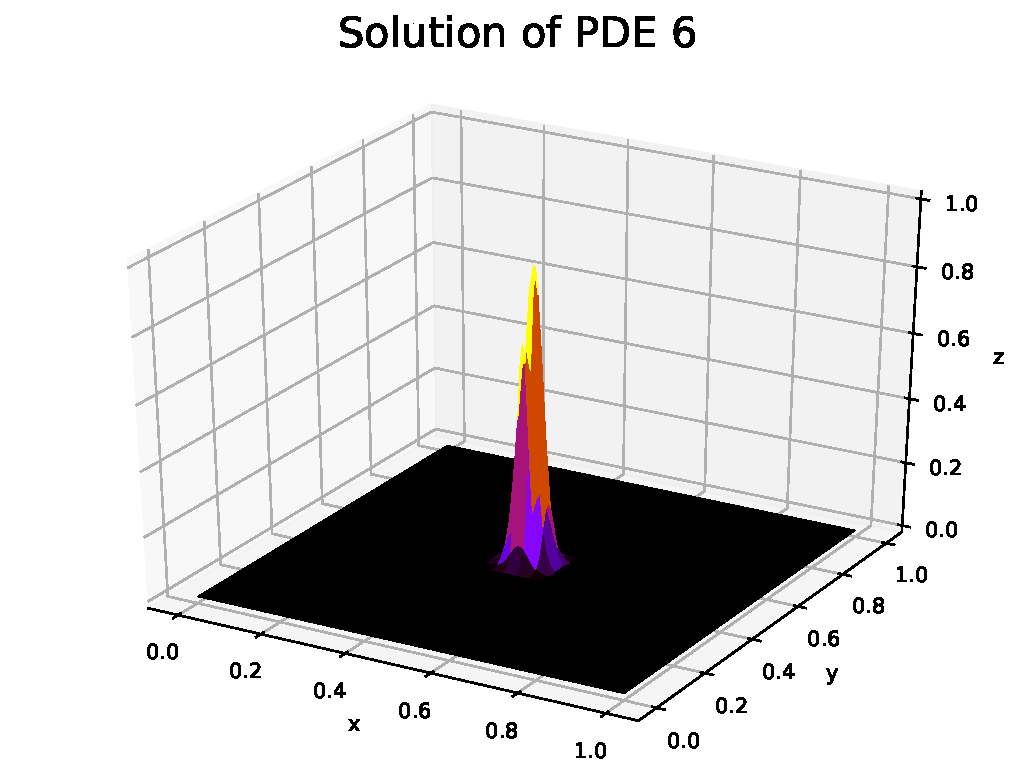
\includegraphics[width=1\textwidth]{../../code/testbed/pde6/sol_pde_6.pdf}
		\caption{Analytical solution \\to \gls{pde} 6.}
		\label{fig:pde6_analytical_solution}
	\end{subfigure}%
	\unterschrift{These wrong solutions are generated with paJADE after $10^6$ \gls{nfe} and represent local optima where JADE gets stuck. }{}{}%
	\label{fig:paJADE_pde6_3D_plot_outlier}
\end{figure}

Corresponding to these 3D plots, the kernel bar plot is depicted in figure \ref{fig:paJADE_pde6_kernel_bar_plot_outlier1} and \ref{fig:paJADE_pde6_kernel_bar_plot_outlier2}. The kernel bar plot connects the decline of the fitness value with the adaption of the kernel number. Darker areas show a strong decline of the best fitness value over generations, lighter areas represent stagnation. A green bar indicates an increment by one kernel. Contrary, the red bar expresses a decrement by one kernel. This shows how figure \ref{fig:pajade_pde6_3D_plot_outlier1} is created by increasing the kernel count, although one kernel should be sufficient. Similar, figure \ref{fig:pajade_pde6_3D_plot_outlier2} consists of a single kernel, where a local optimum is exploited. Both false solutions occur twice within the 20 replications. 

\begin{figure}[H]
	\centering
	\noindent\adjustbox{max width=1\linewidth}{
		
\includegraphics[width=\textwidth]{../../code/experiments/experiment_2/pde6_kernel_bar_plot_outlier1.pdf}
	}
	\unterschrift{Kernel bar plot of the false solution, represented in figure \ref{fig:pajade_pde6_3D_plot_outlier1}}{}{}
	\label{fig:paJADE_pde6_kernel_bar_plot_outlier1}
\end{figure}


\begin{figure}[H]
	\centering
	\noindent\adjustbox{max width=1\linewidth}{
		
\includegraphics[width=\textwidth]{../../code/experiments/experiment_2/pde6_kernel_bar_plot_outlier2.pdf}
	}
	\unterschrift{Kernel bar plot of the false solution, represented in figure \ref{fig:pajade_pde6_3D_plot_outlier2}}{}{}
	\label{fig:paJADE_pde6_kernel_bar_plot_outlier2}
\end{figure}

\end{document}